\documentclass[12pt,letterpaper]{article}
\usepackage[utf8]{inputenc}
\usepackage[spanish]{babel}
\usepackage{graphicx}
\usepackage[left=2cm,right=2cm,top=2cm,bottom=2cm]{geometry}
\usepackage{graphicx} % figuras
% \usepackage{subfigure} % subfiguras
\usepackage{float} % para usar [H]
\usepackage{amsmath}
%\usepackage{txfonts}
\usepackage{stackrel} 
\usepackage{multirow}
\usepackage{enumerate} % enumerados
\renewcommand{\labelitemi}{$-$}
\renewcommand{\labelitemii}{$\cdot$}
% \author{}
% \title{Caratula}
\begin{document}

% Fancy Header and Footer
% \usepackage{fancyhdr}
% \pagestyle{fancy}
% \cfoot{}
% \rfoot{\thepage}
%

% \usepackage[hidelinks]{hyperref} % CREA HYPERVINCULOS EN INDICE

% \author{}
\title{Caratula}

\begin{titlepage}
\begin{center}
\large{UNIVERSIDAD PRIVADA DE TACNA}\\
\vspace*{-0.025in}
\begin{figure}[htb]
\begin{center}

\includegraphics[width=4cm]{./Imagenes/logo}
\end{center}
\end{figure}
\vspace*{0.15in}
INGENIERIA DE SISTEMAS  \\

\vspace*{0.5in}
\begin{large}
TEMA:\\
\end{large}

\vspace*{0.1in}
\begin{Large}
\textbf{Test-Driven Development} \\
\end{Large}

\vspace*{0.3in}
\begin{Large}
\textbf{CURSO:} \\
\end{Large}

\vspace*{0.1in}
\begin{large}
BASE DE DATOS II\\
\end{large}

\vspace*{0.3in}
\begin{Large}
\textbf{DOCENTE(ING):} \\
\end{Large}

\vspace*{0.1in}
\begin{large}
 Patrick Jose Cuadros Quiroga\\
\end{large}

\vspace*{0.2in}
\vspace*{0.1in}
\begin{large}
Integrantes: \\
\begin{flushleft}

Marko Antonio RIVAS RIOS          	\hfill	(2016055461) \\
Jorge Luis MAMANI MAQUERA    	           \hfill	(2016055236) \\
Andree Ludwed VELASCO SUCAPUCA	\hfill	(2016055286) \\
Yofer Nain CATARI CABRERA		\hfill	(2017059289) \\
Adnner Sleyder ESPERILLA RUIZ		\hfill	(2015050543) \\
Jesus ESCALANTE ALANOCA           	\hfill	(2015050641) \\

\end{flushleft}
\end{large}
\end{center}

\end{titlepage}


\tableofcontents % INDICE
\thispagestyle{empty} % INDICE SIN NUMERO
\newpage
\setcounter{page}{1} % REINICIAR CONTADOR DE PAGINAS DESPUES DEL INDICE

\section{Patrones de Diseño Composite} 

\textbf{}\\
El patrón de diseño Composite nos sirve para construir estructuras complejas partiendo de otras estructuras mucho más simples, dicho de otra manera, podemos crear estructuras compuestas las cuales están conformadas por otras estructuras más pequeñas.
Para comprender mejor como funciona este patrón imaginemos una casa de ladrillos, las casas como tal no están hecha de una pieza, si observamos las paredes estas esta echas de pequeñas piezas llamadas ladrillos, entonces, el conjunto de estos ladrillos crea paredes, y un conjunto de paredes crean una casa. este ejemplo puede ser aplicado al patrón Composite, y no digo que vayamos a crear una casa con este patrón, sino más bien nos da una idea de cómo trabaja para poder utilizarlo con otros ejemplos.

\begin{flushleft}

\begin{center}
	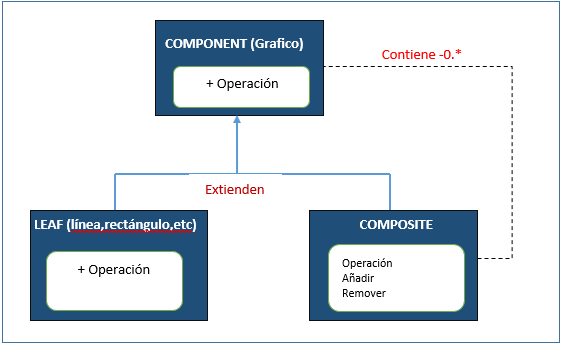
\includegraphics[width=10cm]{./Imagenes/composite1} 
	\end{center}
\begin{itemize}
\textbf{Uso}

El patrón Composite sirve para construir objetos complejos a partir de otros más simples y similares entre sí, gracias a la composición recursiva y a una estructura en forma de árbol.  Esto simplifica el tratamiento de los objetos creados, ya que al poseer todos ellos una interfaz común, se tratan todos de la misma manera. Dependiendo de la implementación, pueden aplicarse procedimientos al total o una de las partes de la estructura compuesta (todo o parte) como si de un nodo final se tratara, aunque dicha parte esté compuesta a su vez de muchas otras.

\textbf{}\\
\textbf{Aplicación}


Usar el patrón COMPOSITE cuando:


  \item Se quiere representar jerarquías de objetos todo-parte.
  \item Se quiere ser capaz de ignorar la diferencia entre objetos individuales y composiciones de objetos.  Los clientes tratarán a todos los objetos de la estructura compuesta uniformemente.

\end{itemize} 

\textbf{}\\
\textbf{}\\
\textbf{}\\
\textbf{}\\
\textbf{}\\
\textbf{}\\
\textbf{Estructura}

\textbf{}\\ 
\textbf{}\\ 

\begin{center}
	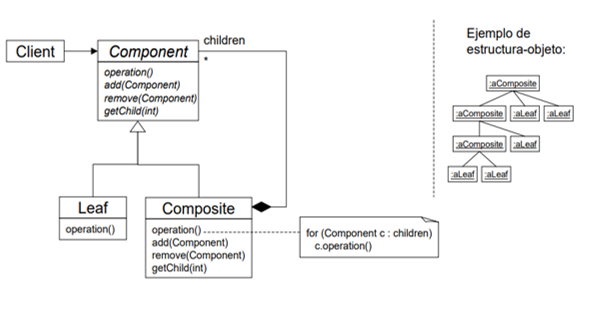
\includegraphics[width=10cm]{./Imagenes/composite2} 
	\end{center}

\textbf{Participantes}

El patrón Composite requiere mínimo de tres componentes para poder existir los cuales son Componente, Leaf o Rama y Composite.

\begin{enumerate}[a)]
        \item \textbf{ Component (Grafico)}
Generalmente es una interface o clase abstracta la cual tiene las operaciones mínimas que serán utilizadas, este componente deberá ser extendido por los otros dos componentes Leaf y Composite. En nuestro ejemplo esto podría representar de forma abstracta un ladrillo o toda la casa (Mas adelante comprenderemos porque)

        \item \textbf{ Leaf o Rama (Línea, Rectángulo, Texto)}
El leaf u hoja representa la parte más simple o pequeña de toda la estructura y este extiende o hereda de Component. En nuestro ejemplo, este representaría un ladrillo de nuestra casa.

	\item \textbf{Composite (Dibujo)}
Aquí es donde está la magia de este patrón, ya que el composite es una estructura conformada por otros Composite y Leaf, los Composite tiene los métodos add  (añadir) y remove (remover) los cuales nos permiten agregar objetos de tipo Component, Sin embargo, el Componente es por lo general un Interface o Clase abstracta  por lo que se puede agregar objetos de tipo Composite o Leaf.   Desde el punto de vista del ejemplo de la casa el Composite podría representar un conjunto de ladrillos o la casa completa, Esto desde luego sería agregando varias Ladrillo(Leaf) al Composite para crear una Pared.

	\item \textbf{ Client}
Es la entidad que hará uso del objeto compuesto.
    \end{enumerate}

\textbf{}\\ 
\textbf{}\\ 
\textbf{}\\ 
\textbf{}\\ 
\textbf{}\\ 
\textbf{}\\ 
\textbf{}\\ 
\textbf{}\\ 
\textbf{}\\ 
\textbf{EJEMPLO DE ESTUDIO DEL PATRON COMPOSITE}
Imaginemos un sistema de puntos de venta, en el cual se le pueden vender al cliente una serie de productos, estos productos pueden ser productos simples (Leaf) o paquetes (Composite).  El sistema permitirá crear “Ordenes de Ventas”, las cuales están compuestas por 1 o muchos productos.

\begin{center}
	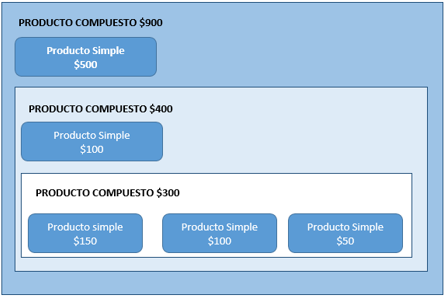
\includegraphics[width=10cm]{./Imagenes/composite3} 
	\end{center}

En la imagen se muestra de forma gráfica cómo está compuesto un paquete.  Los paquetes están creados a partir de un conjunto de productos simples y otros paquetes por lo que el precio de un paquete está calculado por el precio de sus hijos de forma recursiva.  Muestra la estructura de una forma conceptual, sin embargo, la estructura es un poco más compleja, ya que está formado por una estructura de dato llamado “Arbol”

\begin{center}
	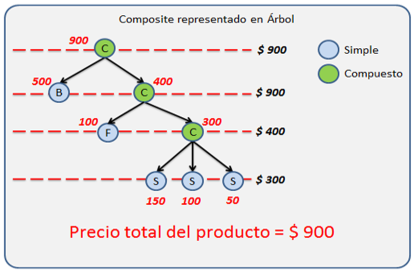
\includegraphics[width=10cm]{./Imagenes/composite4} 
	\end{center}

Esta imagen muestra un solo paquete, está formado de otros productos, simples y compuestos, un compuesto sería otro paquete, el cual tiene dentro más productos simples y como se vio en la figura anterior, el precio de un paquete es calculado por el precio de todos los hijos de forma recursiva.

\textbf{}\\ 
\textbf{}\\
\textbf{}\\
\textbf{}\\
\textbf{}\\
\textbf{}\\

\textbf{CONCLUSION}

\begin{itemize}
\item Define jerarquías de clases hechas de objetos simples y compuestos. 
\item Si el código cliente espera un objeto simple, puede recibir también uno compuesto 
\item Puede hacer el diseño demasiado general. Es complicado restringir el tipo de componentes de un composite.
\item Un paquete es producto compuesto de varios productos simples y otros paquetes.
\item Simplifica el cliente.  Los paquetes y productos simples deberán ser tratados de la misma forma, por lo que deberán tener un padre en común.
\item El precio de un paquete es la suma de todos los productos simples que contenga.
\item El sistema deberá mostrar el total de la Orden y los productos que contiene.
\item Facilita la incorporación de nuevos tipos de componentes


\end{itemize} 





\end{flushleft}
\section{¿Qué es Desarrollo Orientado A Pruebas (TDD)?} 
\textbf{}\\
Esta técnica llamada TDD (Test Driven Development), se puede definir como un proceso de desarrollo de software que se basa en la idea de desarrollar unas pequeñas pruebas, codificarlas y luego refactorizar el código que hemos implementado anteriormente.
Podemos decir que esta técnica e implementación de software está dentro de la metodología XP donde deberíamos de echarle un ojo a todas sus técnicas, tras leer varios artículos en un coincido con Peter Provost con un diseño dirigido o implementado a base de ejemplos hubiese sido mejor pero TDD se centra en 3 objetivos claros:

\begin{flushleft}

\begin{itemize}

	\item Una implementación de las funciones justas que el cliente necesita y no más, solamente las funciones que necesitamos, estoy cansado de duplicar dichas funciones para que hagan lo mismo

	 Mínimos defectos en fase de producción

	\item Producción de software modular y sobre todo reutilizable y preparado para el cambio


\textbf{}\\
Esta técnica se basa en la idea de realizar unas pruebas unitarias para un código que nosotros debemos construir, Nuestro TDD lo que nos dice es que primero los programadores debemos realizar una prueba y a continuación empezar a desarrollar el código que la resuelve.
El método que debemos seguir a para empezar a utilizar TDD es sencillo, Nos sirve para elegir uno de los requisitos a implementar, buscar un primer ejemplo sencillo, crear una prueba, ejecutarla e implementar el código mínimo para superar dicha prueba.
Obviamente la gracia de ejecutar la prueba después de crearla es ver que esta falla y que será necesario hacer algo en el código para que esta pase.
El ciclo de desarrollo de TDD es empezar la prueba, en test realizar un test, revisar el código y pasar el refactor.

\textbf {Crear la prueba o test}
\item Ejecutar los tests: falla (ROJO)
\item Crear código específico para resolver el test
\item Ejecutar de nuevo los tests: pasa (VERDE)
\item Refactorizar el código
\item Ejecutar los tests: pasa (VERDE)

\textbf {Personalmente, añadiría lo siguiente:}
\item Incrementa la productividad.
\item Nos hace descubrir y afrontar más casos de uso en tiempo de diseño.
\item La jornada se hace mucho más amena.
\item Uno se marcha a casa con la reconfortante sensación de que el trabajo está bien hecho.


Ahora bien, como cualquier técnica, no es una varita mágica y no dará el mismo resultado a un experto arquitecto de software que a un programador junior que está empezando. Sin embargo, es útil para ambos y para todo el rango de integrantes del equipo que hay entre uno y otro.
Es una técnica a tener en cuenta en el desarrollo web y sobre todo en el desarrollo de ingeniería software donde debemos tener en cuenta muchos fallos antes de pasar a producción.



\end{itemize} 


\end{flushleft}
\section{Ventajas del TDD} 

\textbf{}\\
\begin{flushleft}

\begin{itemize}
  \item Puedes mejorar el código de tu aplicación en cualquier momento sin miedo a que dañes algo, ya que las pruebas ya las tienes listas y deberán pasar siempre.

  \item Los test que realizamos sobre las interfaces de nuestra app no siempre son completos, generalmente es lo que nos acordamos probar.

  \item Los equipos de testing, development y analyst serán más felices.

  \item La lectura del código será mucho mejor al tener ejemplos de uso (las pruebas).


\end{itemize} 










\end{flushleft}
\section{¿Qué es el Desarrollo Dirigido por Tests? (TDD)} 
\textbf{}\\
\begin{flushleft}
El Desarrollo Dirigido por Tests (Test Driven Development), al cual me referiré como TDD, es una técnica de diseño e implementación de software,
TDD es una técnica para diseñar software que se centra en tres pilares fundamentales.

\begin{itemize}


\item  La implementación de las funciones justas que el cliente necesita y no más.

\item  La minimización del número de defectos que llegan al software en fase de producción.

\item La producción de software modular, altamente reutilizable y preparado para el cambio.



MockObjects y TDD en .Net Framework


El desarrollo guiado por pruebas es una práctica que está cambiando la forma en la que se desarrolla Software de calidad. Para poder aplicarla correctamente es necesario el dominio de los MockObjects para aislarse de las dependencias externas.


Pruebas Unitarias y Simulación de objetos

Otra alternativa para realizar la simulación, consiste en conseguir probar el código unitariamente, esto significa aislarse de todos los recursos externos, es decir no depender de la infraestructura de red, o de un determinado entorno, o incluso del proceso que ejecutará nuestro código cuando esté en producción. Cargaremos las pruebas y el código a probar en un proceso encargado de gestionar la ejecución de las pruebas.

\end{itemize} 


\end{flushleft}
\section{Profundizar tema} 
\textbf{}\\
\begin{flushleft}


\begin{itemize}



	


\end{itemize} 


\end{flushleft}
\section{¿Quién está haciendo TDD realmente?} 
\textbf{}\\
\begin{flushleft}
\begin{center}	
\end{center}
\begin{itemize}
\textbf{1.	 “¿Qué tan ágil es TDD?” }
\textbf{}\\
Desafortunadamente, la tasa de adopción de TDD no es tan alta como debería ser realmente.  La siguiente figura resume los resultados del 2010


\textbf{}\\
 La encuesta proporciona información sobre las estrategias de validación que siguen los equipos que dicen ser ágiles. Sospecho que las tasas de adopción informadas para el desarrollador TDD y la aceptación TDD, 53% y 44% respectivamente, son mucho más realistas que las informadas en mi Encuesta sobre el desarrollo impulsado por pruebas (TDD) .

\textbf{}\\

\begin{center}
    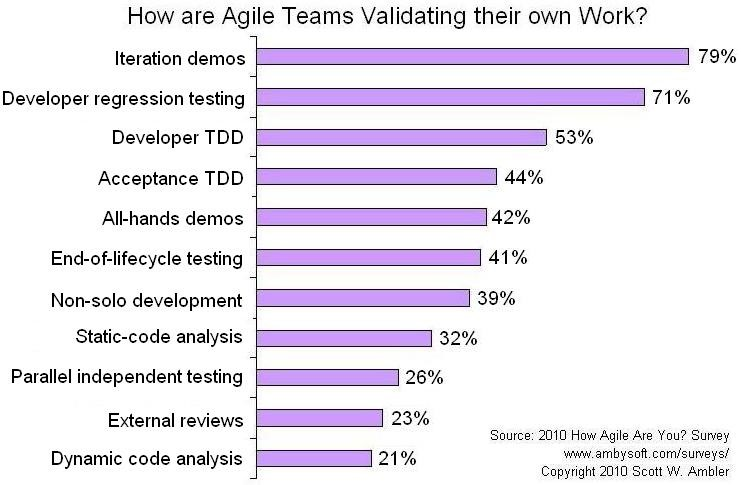
\includegraphics[width=12cm]{./Imagenes/test}
    \end{center}

\end{itemize} 







\end{flushleft}
\section{Webgrafía} 
\textbf{}\\
\begin{flushleft}

\begin{itemize}

	\item https://uniwebsidad.com/libros/tdd/capitulo-2
           \item https://docs.microsoft.com/es-es/previous-versions/bb932285(v=msdn.10)
           \item http://www.conaiisi.unsl.edu.ar/portugues/2013/158-524-1-DR.pdf
           \item https://openwebinars.net/blog/que-es-tdd-test-driven-development/
           \item https://altenwald.org/2009/01/08/desarrollo-orientado-a-pruebas-tdd/
           \item https://uniwebsidad.com/libros/tdd/capitulo-2


\end{itemize} 


\end{flushleft}


\end{document}